\begin{frame}[fragile]

  {\Huge BLAS and LAPACK}

  \vspace{20pt}

  \textbf{Learning objectives:}
  \begin{itemize}
    \item {Motivation for BLAS/LAPACK functions}
    \item {Algorithm Specialization for Applications}
    \item {Calling BLAS/LAPACK functions}
  \end{itemize}

  \vspace{-20pt}
\end{frame}

%==========================================================================
% Slide 2
\begin{frame}[fragile]{KokkosKernels BLAS/LAPACK Interface}

\vspace{-1em}
  \begin{columns}[t,onlytextwidth]
    \column{.50\textwidth}
      \begin{center}
        \textbf{KokkosKernels}
      \end{center}
    \column{.50\textwidth}
      \begin{center}
        \textbf{Vendor Libraries}
      \end{center}
  \end{columns}

%\noindent\makebox[\linewidth]{\rule{\paperwidth}{0.4pt}}
\noindent\rule{4in}{0.4pt}

  \begin{columns}[t,onlytextwidth]
    \column{.45\textwidth}
      \begin{flushleft}
      \vspace{-2em}
        \begin{itemize}
          \item \small{A single interface to vendor BLAS libraries on
          heterogenous computing platforms}
          \item \small{Support user-defined data type e.g., Automatic Differentiation,
          Ensemble, SIMD, types with Kokkos native implementation}
          \item \small{Customized performance solution for certain problem sizes}
          \item \small{Exploring new performance oriented interfaces}
        \end{itemize}
      \end{flushleft}
    \column{.10\textwidth}
    \column{.45\textwidth}
      \begin{flushright}
      \vspace{-2em}
        \begin{itemize}
          \item \small{A user needs to write a different function interface for
          different computing platforms e.g., MKL vs. CUBLAS}
          \item \small{Built-in real/complex data types and column/row major data
          layouts are only supported}
          \item \small{Code is highly optimized; in practice, higher performance is
          obtained from larger problem sizes}
        \end{itemize}
      \end{flushright}
  \end{columns}
\end{frame}

%==========================================================================
% Slide 3
\begin{frame}[fragile]{KokkosKernels BLAS/LAPACK Interface}
  \textbf{Algorithm Specialization for Applications}
  \begin{itemize}
    \item Dot-based GEMM
    \begin{itemize}
	    \item \small{GEMM is used for orthogonalizing Krylov multi-vectors (long skinny matrix)}
      \item \small{This particular problem shape does not perform well on CUBLAS}
      \item \small{Algorithm is specialized for this shape performing multiple dot
      products instead of running standard GEMM algorithms}
    \end{itemize}
    \item Compact Batched BLAS
    \begin{itemize}
      \item \small{Application wants to solve many instances of tiny square block dense
      matrices; e.g., block dimensions of 3, 5, 7, 9, 11, etc.}
      \item \small{Difficult to effectivley use wide vector length such as AVX512 for
      this small problem size}
      \item \small{A pack of block matrices are inter-leaved and solved simultaneously
      using vector instructions}
      \item \small{Code is trivially vectorized 100\% for the applied BLAS and LAPACK operations}
    \end{itemize}
  \end{itemize}
\end{frame}

%==========================================================================
% Slide 3
\begin{frame}[fragile]{KokkosKernels BLAS/LAPACK Interface}
  \textbf{Algorithm Specialization for Applications}
  \begin{itemize}
    \item Extended Blas 1 interface: see axpby, update (a, c, b, y, g, z)
    \begin{itemize}
      \item $y[i] = g*z[i] + b*y[i] + a*x[i]$
      \item Trilinos Tpetra interface used in Belos iterative solvers
    \end{itemize}
    \item See the wiki page for complete list of functions
    \begin{itemize}
      \item https://github.com/kokkos/kokkos-kernels/wiki
    \end{itemize}
  \end{itemize}
  \vspace{10pt}
  \begin{center}
    \framebox{\parbox[t][1.0cm]{9.0cm}{
      \centering
      \item KokkosKernels interacts with application teams and provides custom 
      performance solutions for their needs
    }}
  \end{center}
\end{frame}

%==========================================================================
% Begin NDE
% Slide 5
\begin{frame}[fragile]{KokkosKernels BLAS/LAPACK Interface}

\textbf {Recall the Kokkos Inner Product exercise:}

\begin{columns}[t,onlytextwidth]
  \column{.50\textwidth}
\begin{itemize}
%  \item Recall the Kokkos Inner Product exercise:
  \item Inner product $<y,A*x>$
  \begin{itemize}
    \item $y$ is $Nx1$, $A$ is $NxM$,\\ $x$ is $Mx1$
  \end{itemize}
  \item Early exercise code looked like

  \begin{code}[keywords={double,parallel_reduce,for,int}]
double result = 0;
Kokkos::parallel_reduce("yAz", N,
    KOKKOS_LAMBDA (int j, double &update) {
      double temp2 = 0;
      for (int i = 0; i < M; ++i) {
        temp2 += A(j, i) * x(i);
      }
      update += y(j) * temp2;
  }, result);
  \end{code}

\end{itemize}

  \column{.50\textwidth}
  \begin{flushright}
    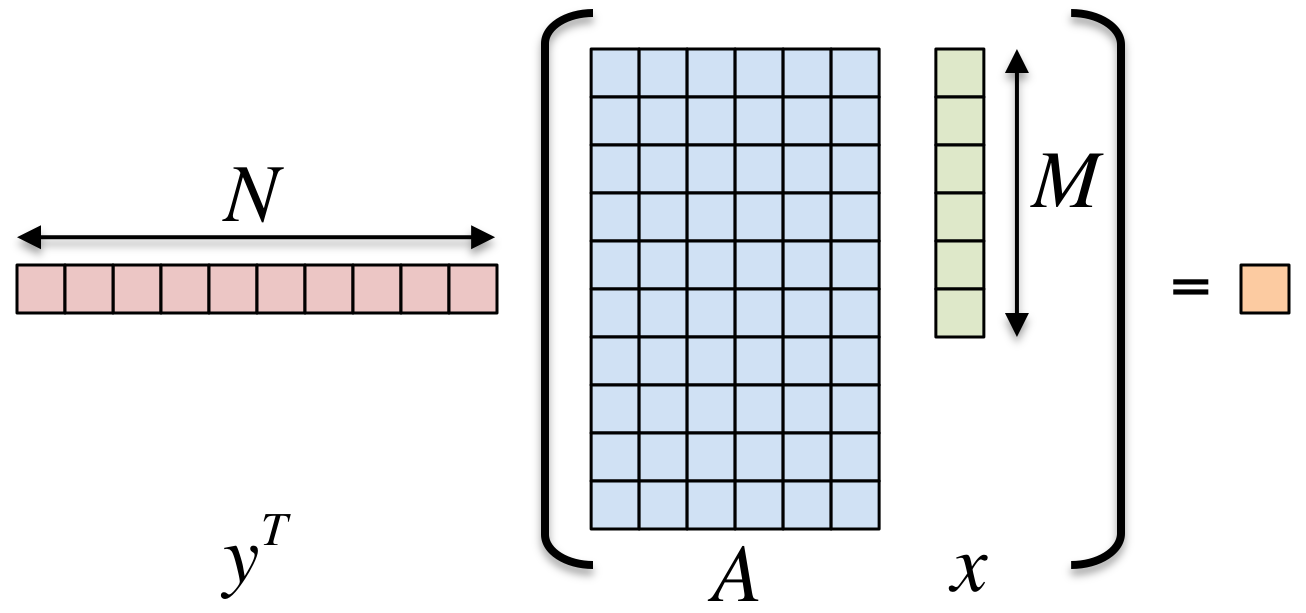
\includegraphics[width=0.85\textwidth]{figures/InnerProductExample_annotated}
  \end{flushright}
\end{columns}
\end{frame}

%Slide 6

\begin{frame}[fragile]{KokkosKernels BLAS/LAPACK Interface}

\textbf {This can be naturally expressed as two BLAS operations:} \\
In Matlab notation:
\vspace{-2em}

\begin{columns}[t,onlytextwidth]
  \column{.50\textwidth}
  \begin{center}
  \begin{code}[keywords={double,parallel_reduce,for,int}]
     // 1. gemv:
     Ytmp = A * x
  \end{code}
  \\
  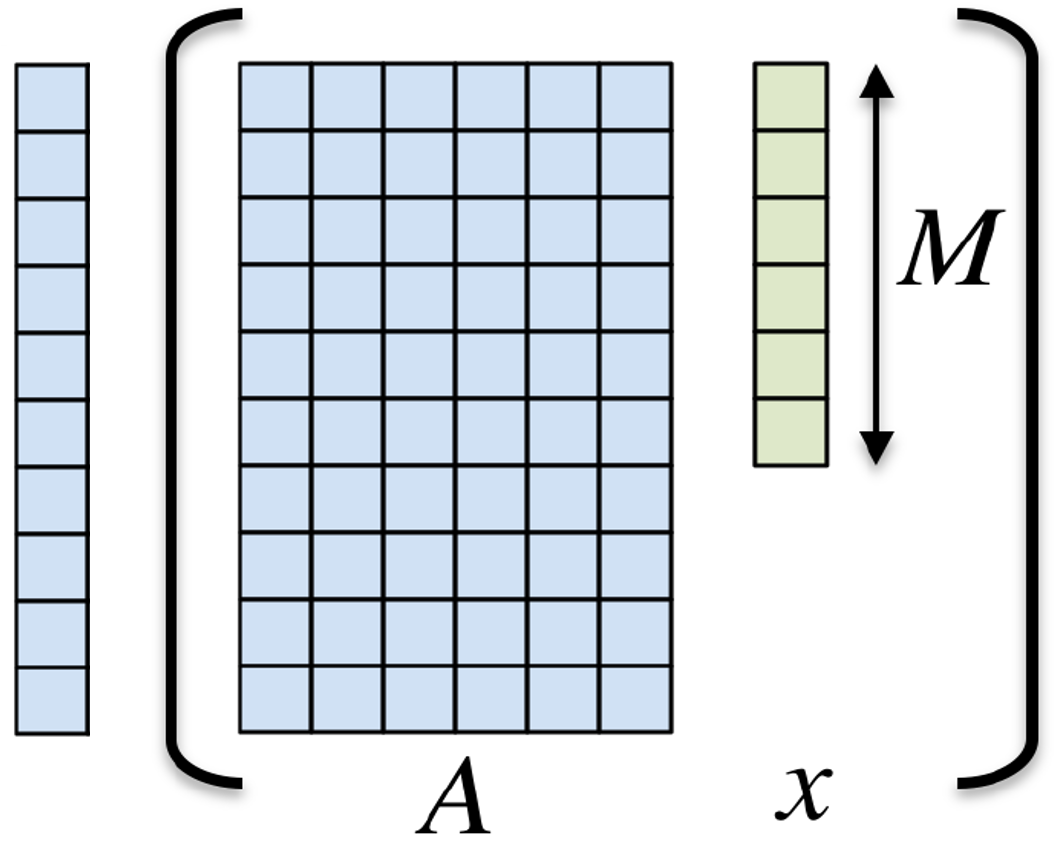
\includegraphics[width=0.5\textwidth]{figures/BLAS-A_times_x_res}
  \end{center}


  \column{.50\textwidth}
  \begin{center}
  \begin{code}[keywords={double,parallel_reduce,for,int}]
     // 2. dot:
     result = y'*Ytmp
  \end{code}
  \\
  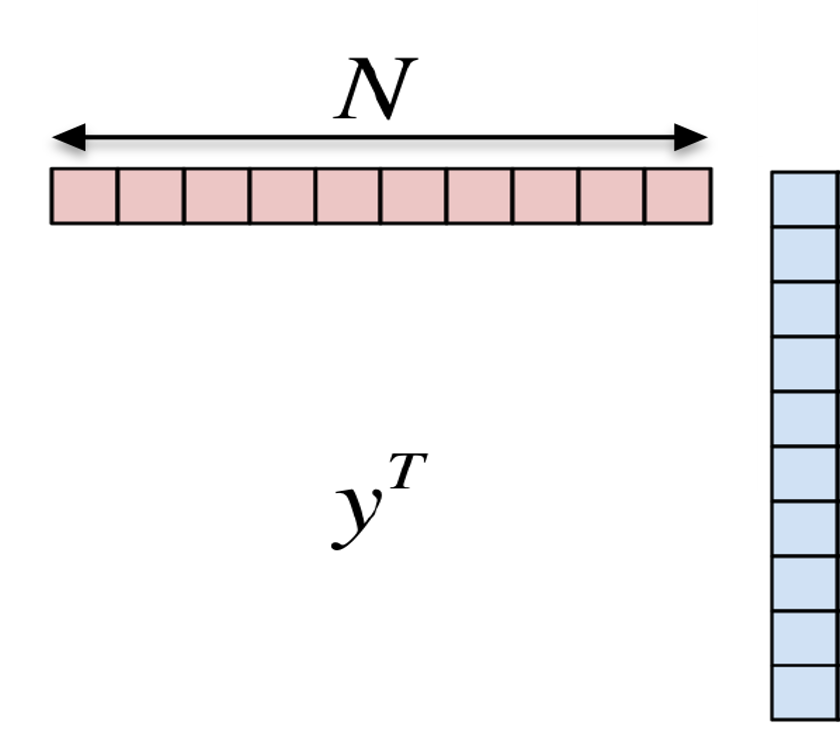
\includegraphics[width=0.5\textwidth]{figures/BLAS-y_dot_tmp}
  \end{center}
\end{columns}
\vspace{5pt}
\small{Different function signatures and APIs are used by different vendors}
\\
\small{  e.g., on Cuda: cublasDgemv and cublasDdot}
\end{frame}

% Slide 7

\begin{frame}[fragile]{KokkosKernels BLAS Interface: GEMV}

%\textbf {KokkosBLAS::gemv}

\begin{code}[basicstyle=\large, keywords={double,gemv,dot}]
KokkosBlas::gemv (mode, alpha, A, x, beta, y);
\end{code}

\textbf {Interface:}

\begin{itemize}
  \item mode [in] 
  \begin{itemize}
    \item "N" for non-transpose
    \item "T" for transpose
    \item "C" for conjugate transpose.
  \end{itemize}
  \item alpha [in] Input coefficient of A*x
  \item A [in] Input matrix, as a 2-D Kokkos::View
  \item x [in] Input vector, as a 1-D Kokkos::View
  \item beta [in] Input coefficient of y
  \item y [in/out] Output vector, as a nonconst 1-D Kokkos::View
\end{itemize}

\end{frame}

% Slide 8

\begin{frame}[fragile]{KokkosKernels BLAS Interface: DOT}

\begin{code}[basicstyle=\large, keywords={double,gemv,dot}]
result = KokkosBlas::dot(x,y);
\end{code}

\textbf {Single Interface:}

\begin{itemize}
  \item x [in] Input vector, as a 1-D Kokkos::View
  \item y [in] Input vector, as a 1-D Kokkos::View
  \item result [out] Scalar result on host
  \item This interface calls Kokkos::fence on all execution spaces
\end{itemize}

\begin{code}[basicstyle=\large, keywords={double,gemv,dot}]
KokkosBlas::dot(r,x,y);
\end{code}

\textbf {Single and Multi-vector Interface:}

\begin{itemize}
  \item x [in] Input (multi-)vector, as a 1-D or 2-D Kokkos::View
  \item y [in] Input (multi-)vector, as a 1-D or 2-D Kokkos::View
  \item r [in/out] Output result, as a rank-0 or 1-D Kokkos::View
  \item This interface is non-blocking.
\end{itemize}

\end{frame}


%==========================================================================
% Slide 9
\begin{frame}[fragile]{KokkosKernels BLAS/LAPACK Interface}

\vspace{-1em}

  \begin{columns}[t,onlytextwidth]
    \column{.50\textwidth}
      \begin{center}
        \textbf{KokkosKernels:}
      \end{center}
    \column{.50\textwidth}
      \begin{center}
        \textbf{User implementation:}
      \end{center}
  \end{columns}

%\noindent\makebox[\linewidth]{\rule{\paperwidth}{0.4pt}}
\noindent\rule{4in}{0.4pt}

  \begin{columns}[t,onlytextwidth]
    \column{.45\textwidth}
      \begin{flushleft}
      \vspace{-2em}
  \begin{code}[keywords={View,double,gemv,dot}, basicstyle=\tiny, breaklines=true]
Kokkos::View<double*> tmp("tmp", N);

KokkosBlas::gemv("N",alpha,A,x,beta,tmp);


double result = 0;

result = KokkosBlas::dot(y,tmp);
  \end{code}
      \end{flushleft}
    \column{.10\textwidth}
    \column{.45\textwidth}
      \begin{flushright}
      \vspace{-2em}
  \begin{code}[keywords={parallel_reduce,for,int,double}, basicstyle=\tiny, breaklines=true]
double result = 0;
Kokkos::parallel_reduce("yAx", N, 
 KOKKOS_LAMBDA (int j, double &update) { 
  double temp2 = 0;
   for (int i = 0; i < M; ++i) { 
     temp2 += A(j, i) * x(i);
   }
   update += y(j) * temp2;
 }, result);
  \end{code}
      \end{flushright}
  \end{columns}

\noindent\rule{4in}{0.4pt}

\vspace{-0.5em}
  \begin{columns}[t,onlytextwidth]
    \column{.45\textwidth}
      \begin{itemize}
        \vspace{-1em}
        \item{\scriptsize{Uses two BLAS functions}}
        \item{\scriptsize{Optionally interface to optimized vendor libraries}}
        \item{\scriptsize{For certain matrix shapes may choose specialized code path for performance}}
      \end{itemize}
    \column{.10\textwidth}
    \column{.45\textwidth}
      \begin{itemize}
        \vspace{-1em}
        \item{\scriptsize{Exploits a single level of parallelism only i.e., internal temp2 is summed sequentially}}
        \item{\scriptsize{Matrix-vector multiplication and dot product are fused in a single kernel}}
      \end{itemize}
  \end{columns}
\vspace{0.5em}
\scriptsize{Related exercise available at: \verb!Exercises/kokkoskernels/InnerProduct!}
%\item \tiny{\url{https://github.com/kokkos/kokkos-tutorials/tree/main/Exercises/kokkoskernels/InnerProduct/Begin}}

\end{frame}

\begin{frame}[fragile]{Summary}

  \textbf{Summary: BLAS/LAPACK}
  \begin{itemize}
  \item \small{Single interface for heterogeneous computing platforms}
  \item \small{Optimized vendor library interface when it is available}
  \item \small{Specialization of algorithms corresponding to application needs}
  \item \small{Native implementation supports strided data layout of a matrix}
  \end{itemize}
  
\end{frame}

%==========================================================================
% End NDE
